\section{Differential expression analysis}
Differential expression analysis was performed using the methods described in
\cref{sec:material_dea}: DESeq2 and \gls{ciriquant}.
In the following sections of this chapter, the results of the differential
expression analysis are presented.

\subsection{\Glspl{crna} associated with estrogen receptor expression}

In order to identify potential markers of estrogen levels, the expression of
the 

\begin{figure}[H] \begin{tabular}{cc} \begin{subfigure}{0.5\textwidth}
                 \centering 

                 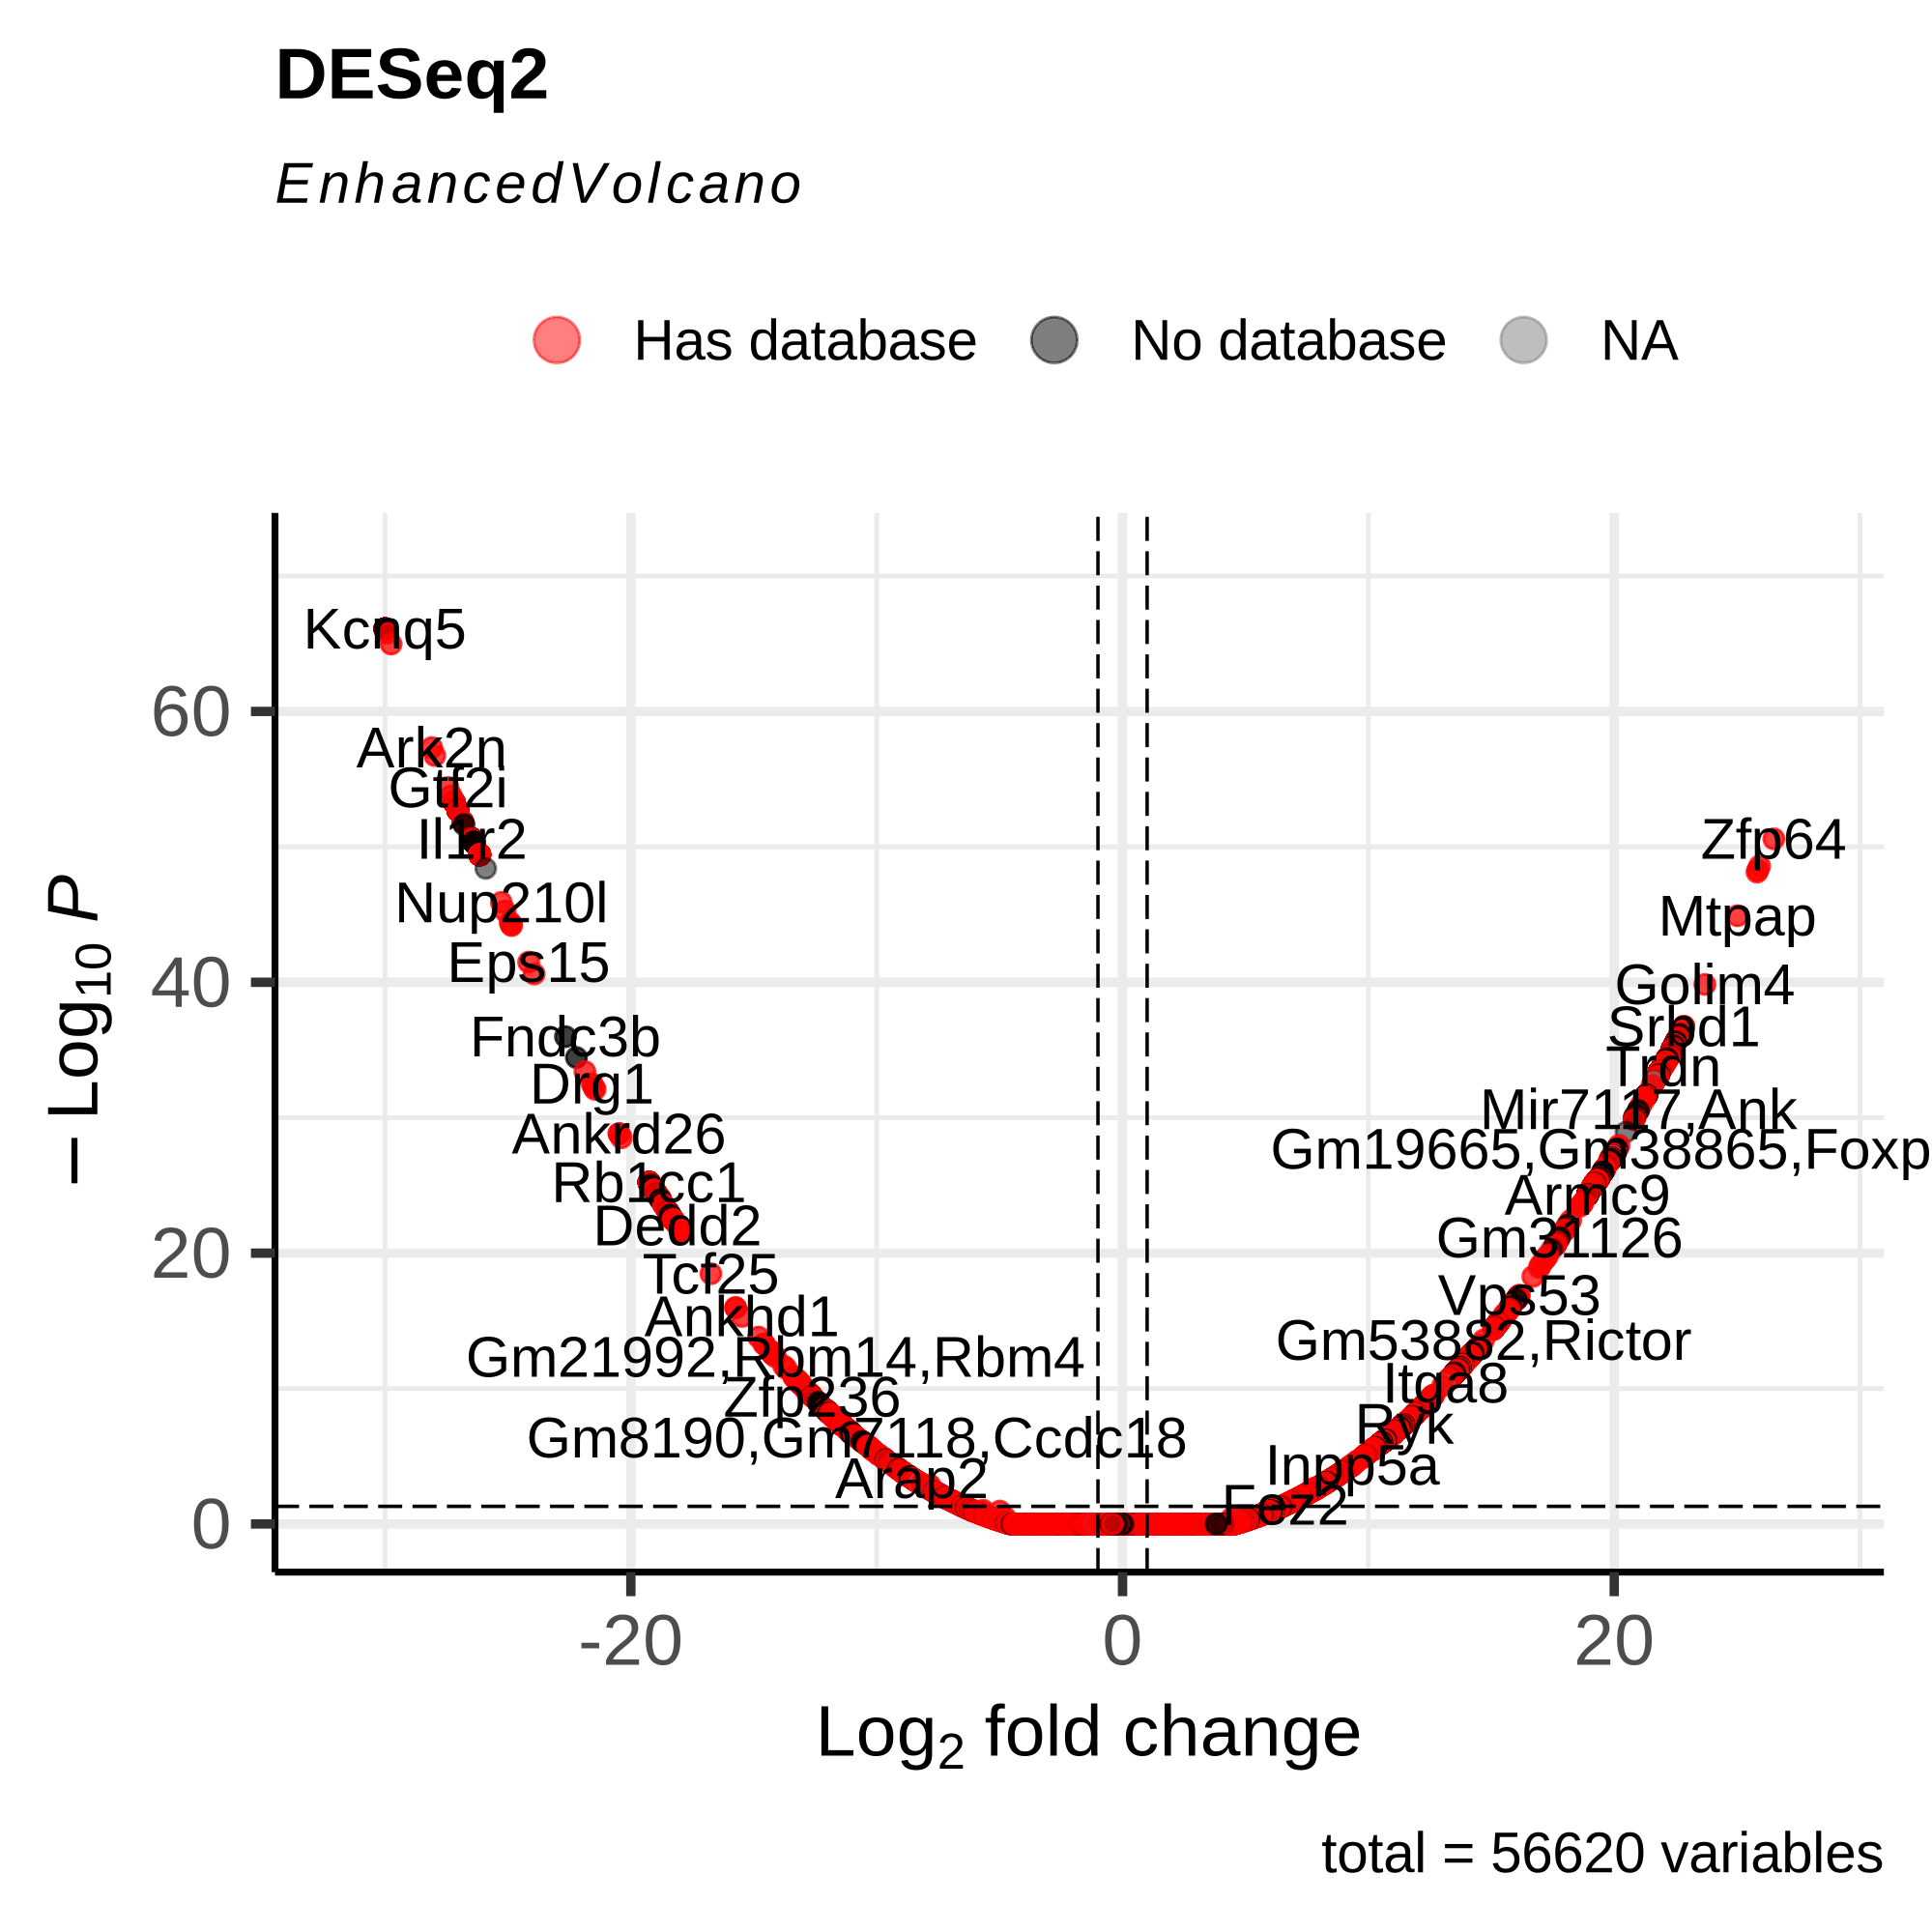
\includegraphics[width=\linewidth]{chapters/4_results_and_discussion/figures/dea/deseq2/esr1/volcano.png}
                 \caption{Volcano plot based on differential expression analysis using DESeq2.
                     Coloring is based on the presence of a supporting database entry in any of the
                     used databases.
                 } \label{fig:esr1_volcano} \end{subfigure}
        \begin{subfigure}{0.5\textwidth} \centering

            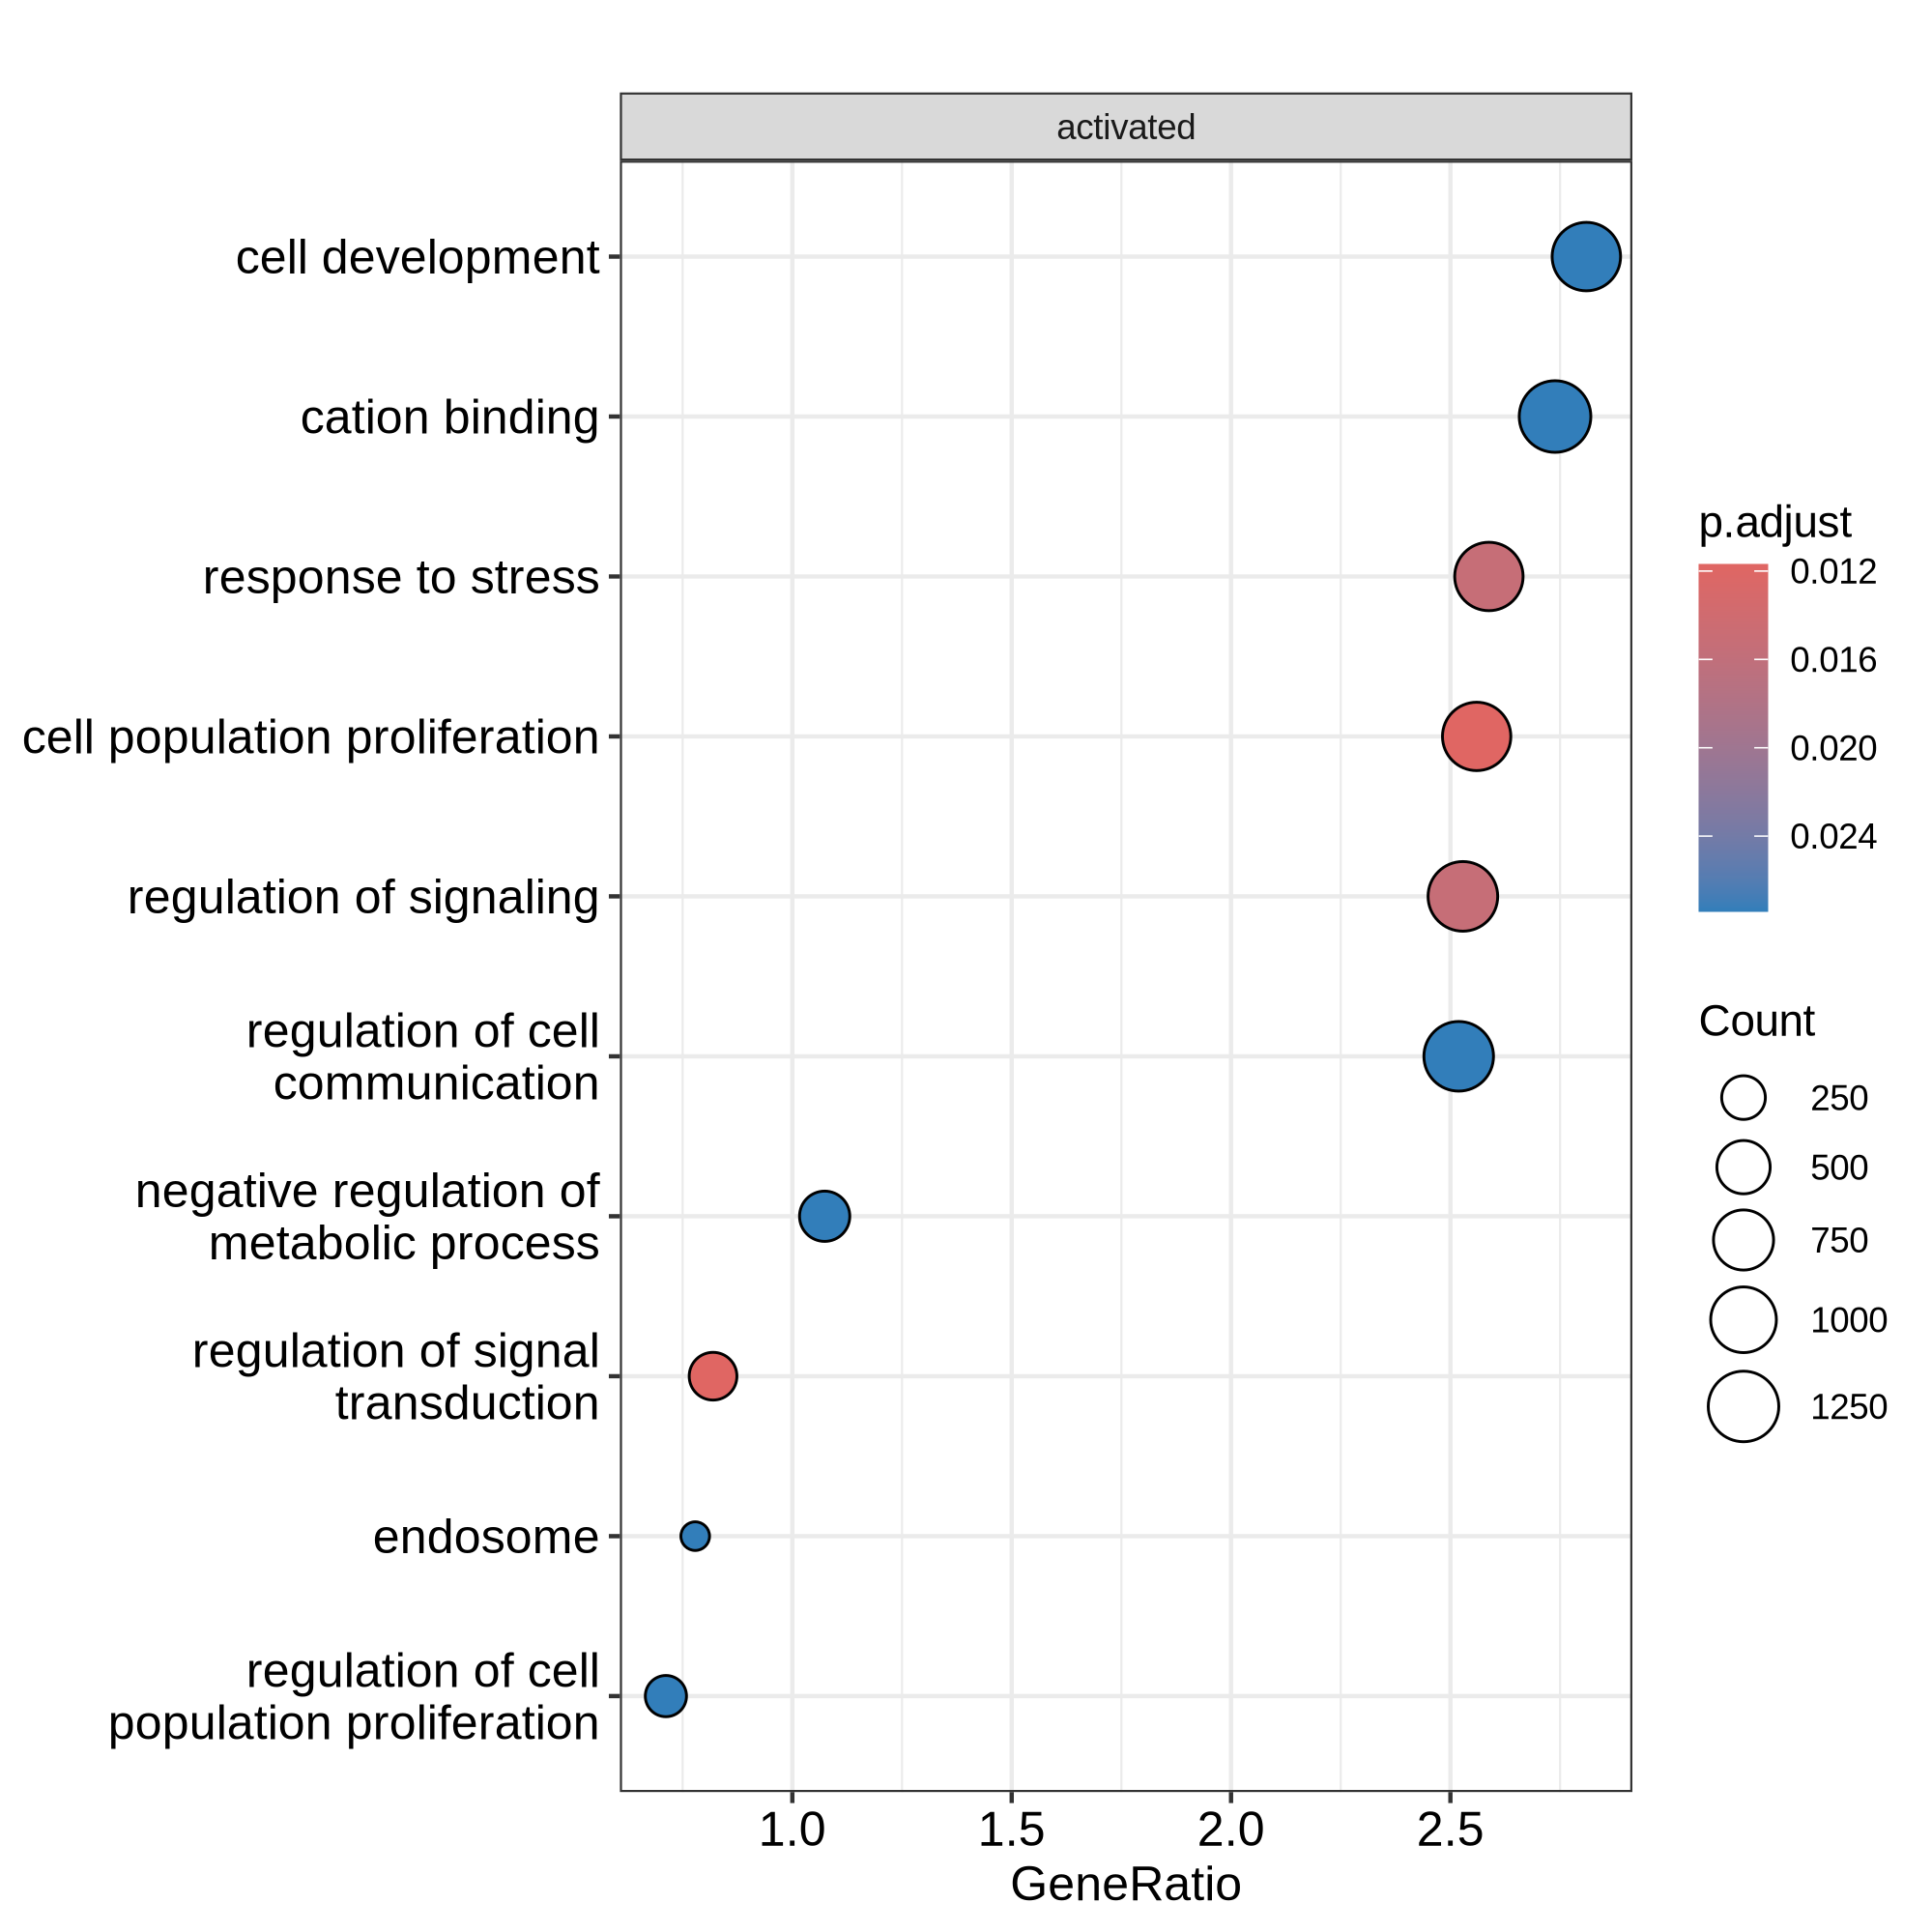
\includegraphics[width=\linewidth]{chapters/4_results_and_discussion/figures/dea/deseq2/esr1/dot.png}
            \caption{Functional enrichment of the host genes of the
                \glspl{crna} marked as significantly associated with \gls{esr1}
                expression.
            }

            \label{fig:esr1_go_terms}
        \end{subfigure}
    \end{tabular}
    \caption{Results of differential expression analysis based on the
        association with \gls{esr1} expression (numeric contrast).
        Expression of the \gls{esr1} gene was determined using the nf-core/rnaseq
        pipeline\supercite{patel_nf-corernaseq_2024}.
        The following design formula was used: $\sim age + transgene + induction + drug
            + esr1$.
        The expression matrix containing all samples was tested for log2 fold changes
        with greater absolute values than 2.
        Benjamini-Hochberg correction\supercite{benjamini_controlling_1995} was used to
        adjust the $p$-values for multiple testing.
        \Glspl{crna} were considered significantly associated with \gls{esr1}
        expression if they had an adjusted $p$-value of less than 0.05.
    }
    \label{fig:dea_esr1}
\end{figure}

\subsection{\Glsfmtshortpl{crna} associated with \glsfmtlong{tam} treatment}

\begin{figure}[H] \begin{tabular}{cc}
        \begin{subfigure}{0.5\textwidth} \centering

            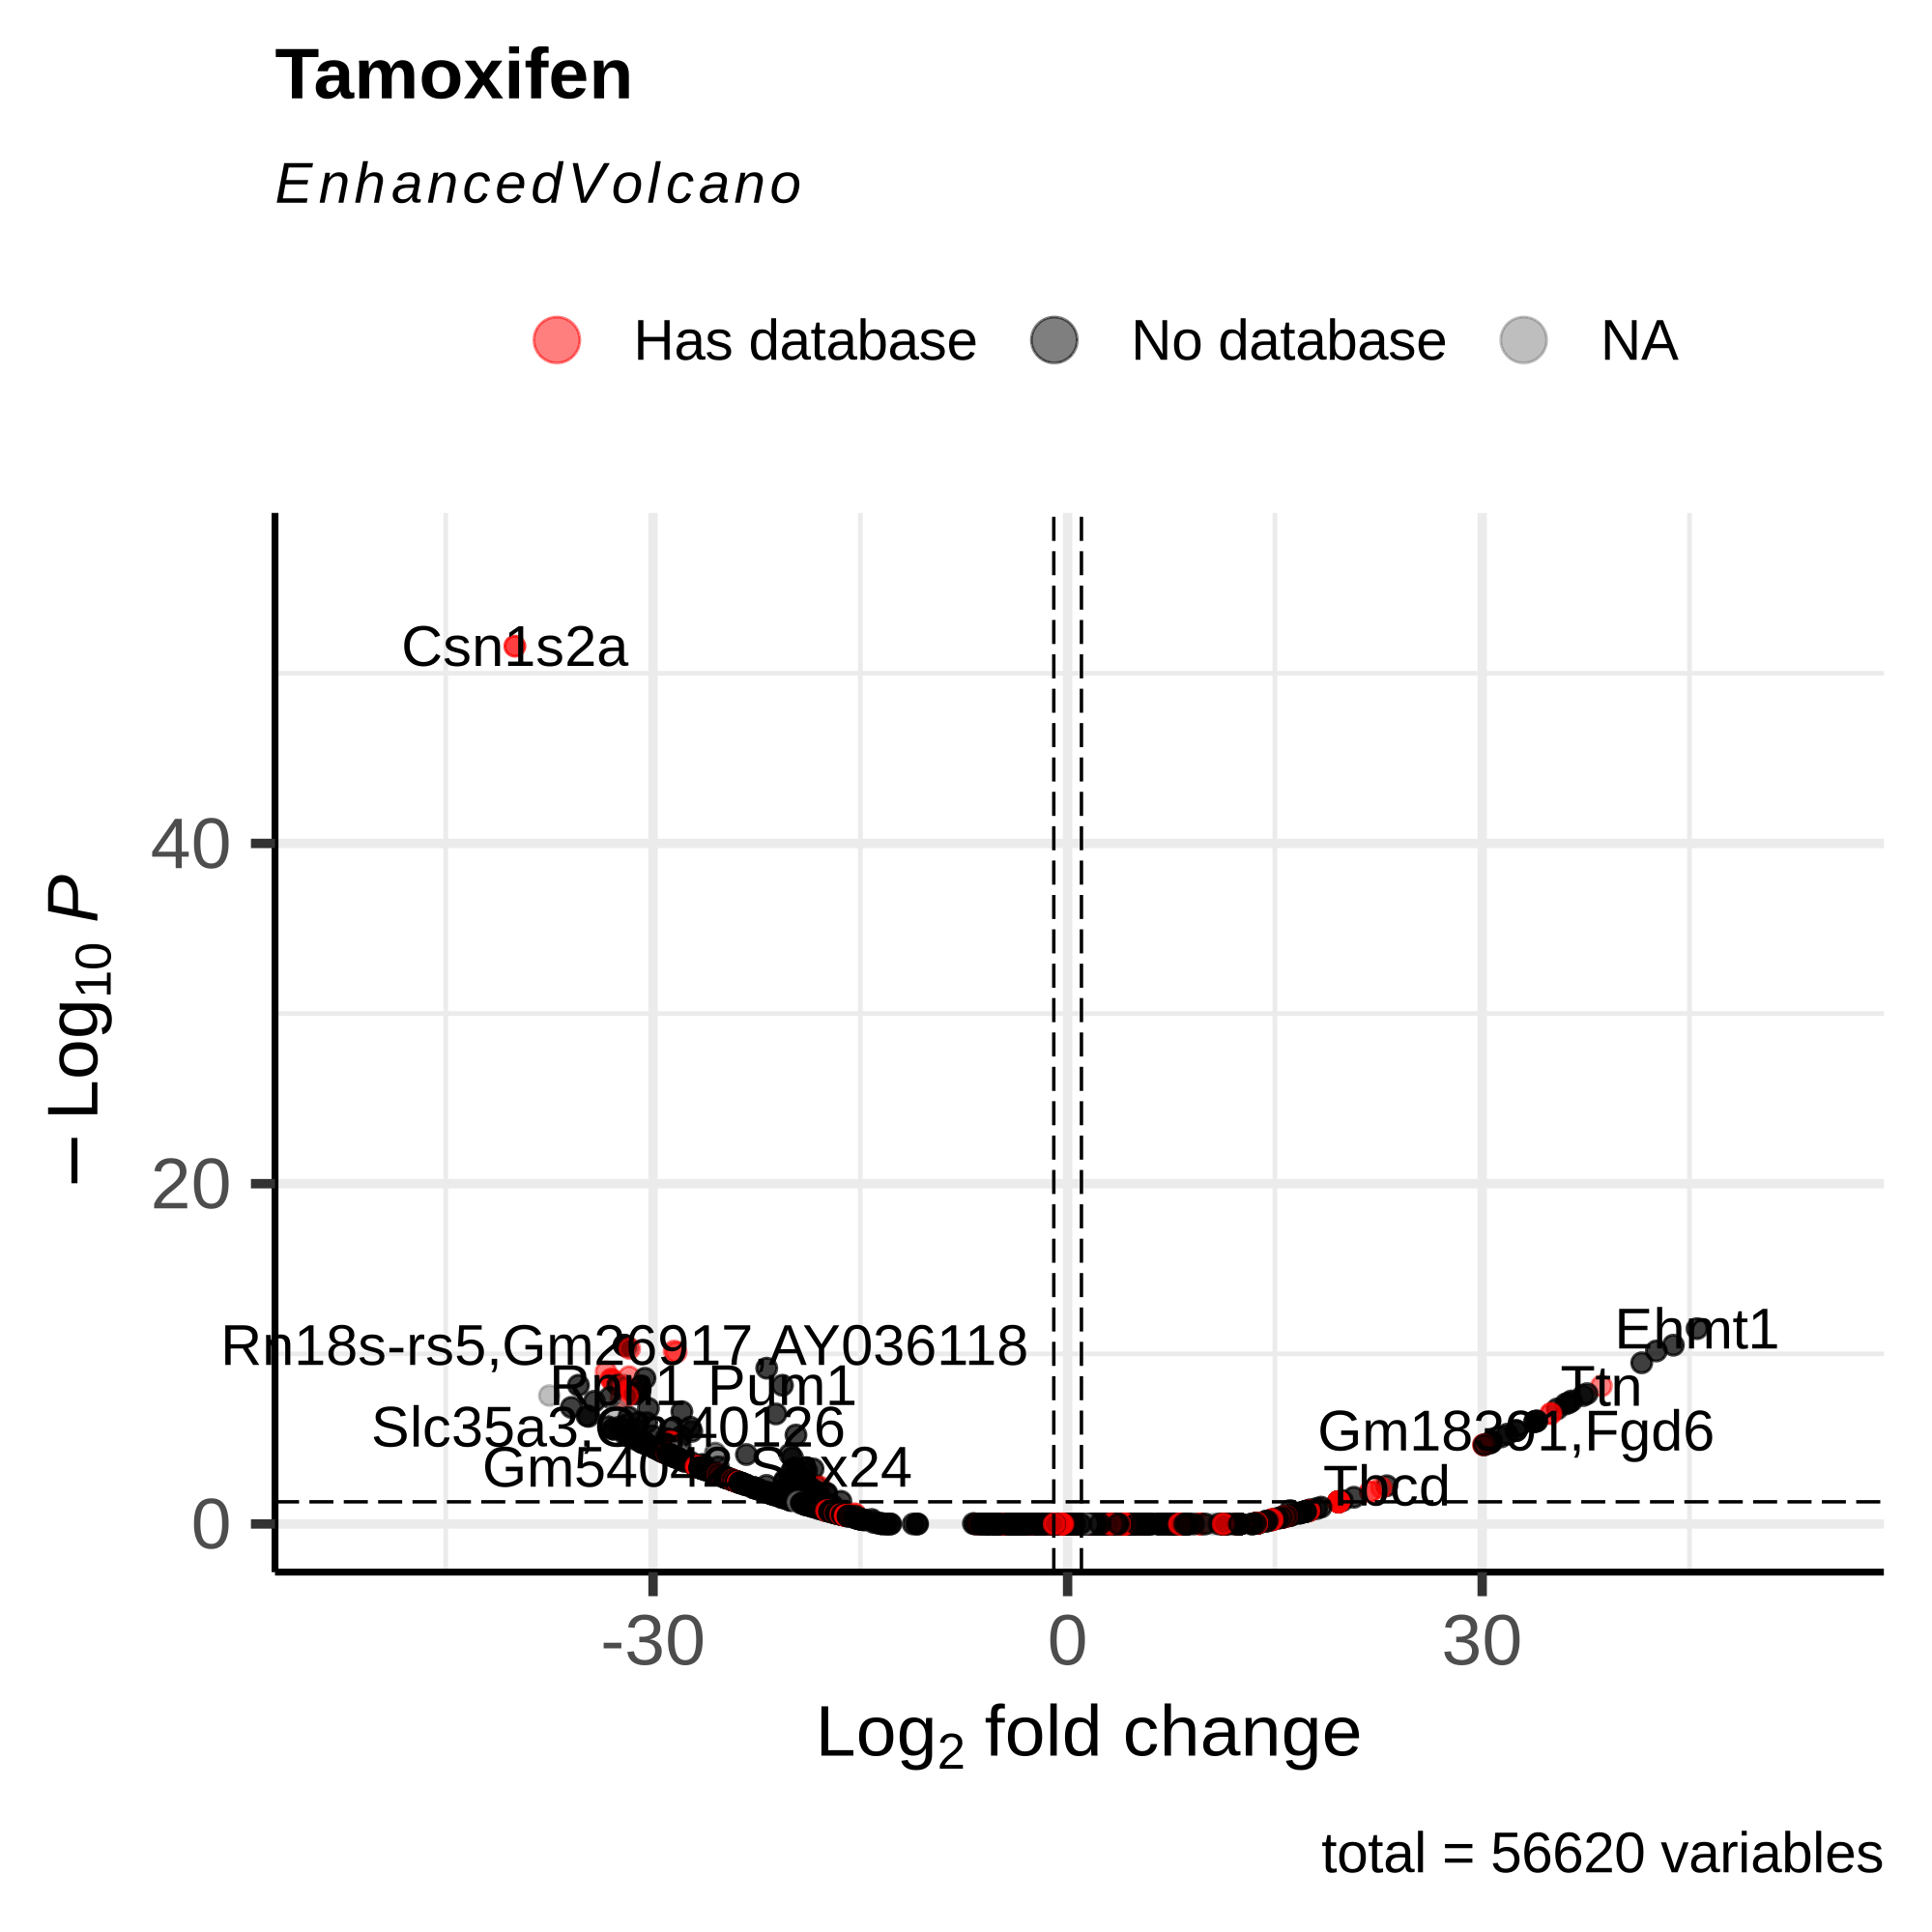
\includegraphics[width=\linewidth]{chapters/4_results_and_discussion/figures/dea/deseq2/tamoxifen/volcano.png}
            \caption{Volcano plot illustrating the differential expression
                results obtained using DESeq2.
                The following design formula was used: $\sim age + transgene + induction +
                    drug$.
                The expression matrix was tested for log2 fold changes with greater absolute
                values than 2.
            }
            \label{fig:tamoxifen_volcano_deseq2}
        \end{subfigure}
        \begin{subfigure}{0.5\textwidth}
            \centering

            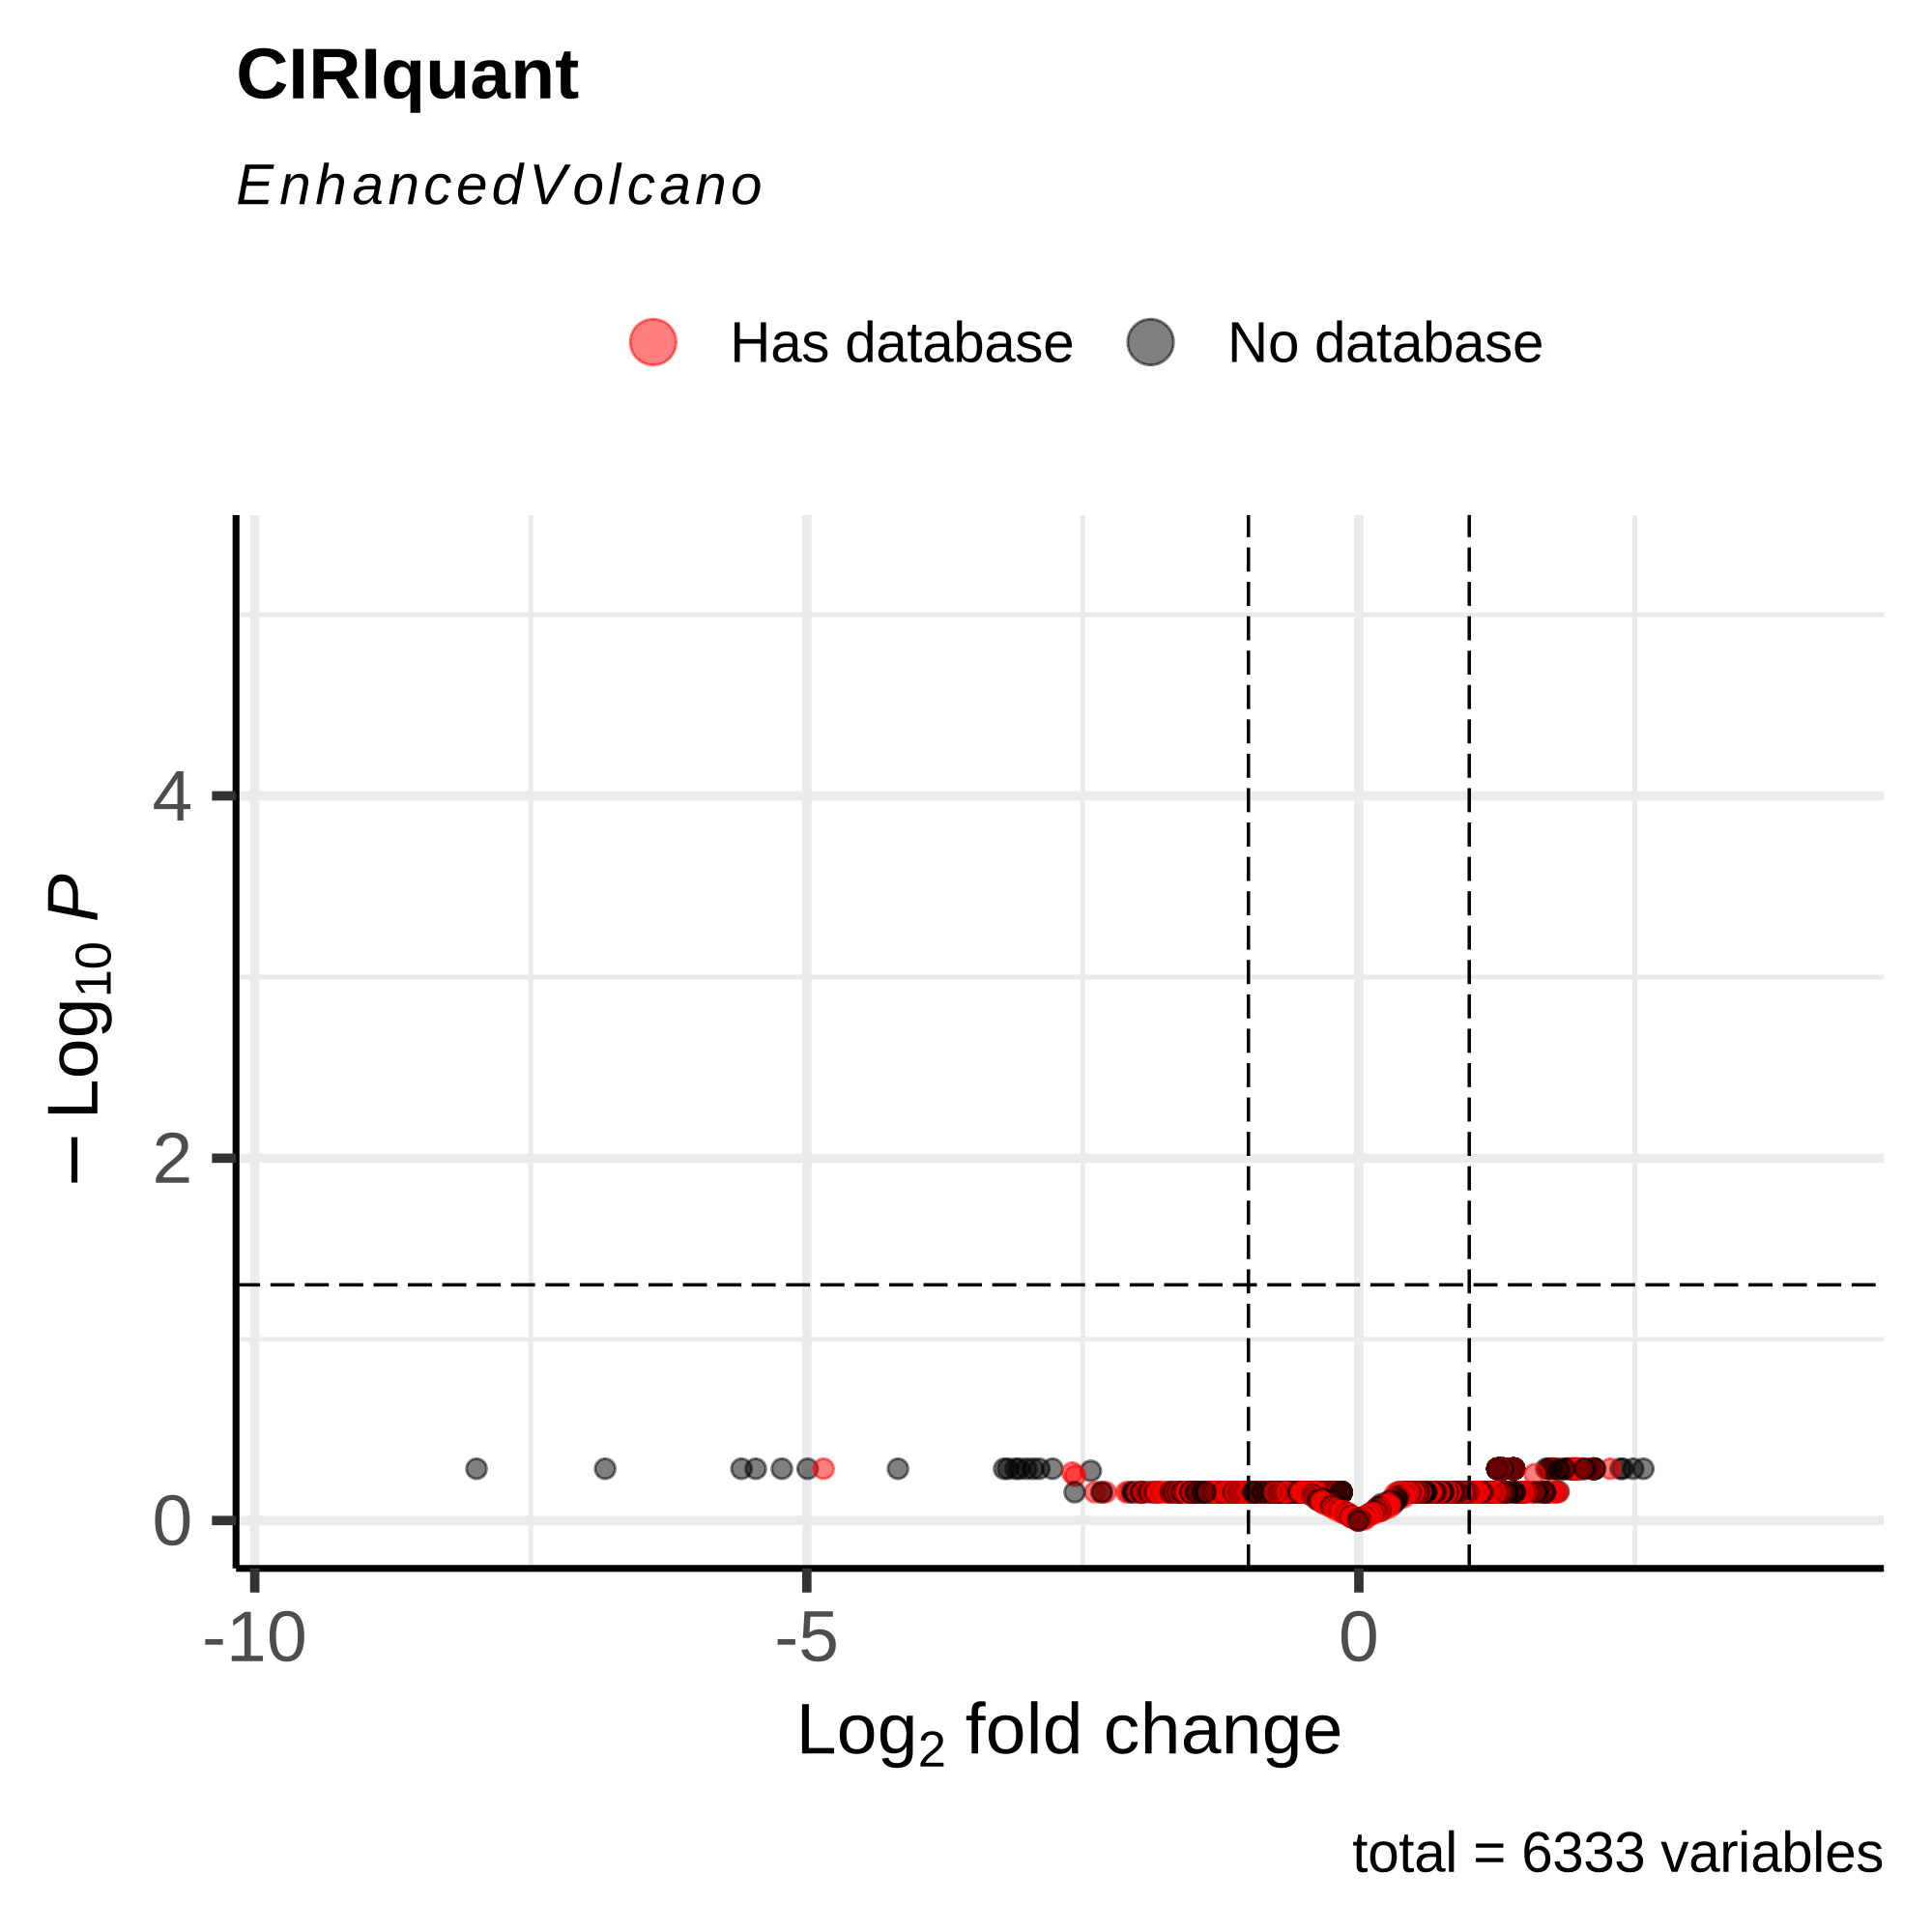
\includegraphics[width=\linewidth]{chapters/4_results_and_discussion/figures/dea/ciriquant/tamoxifen/volcano.png}
            \caption{Volcano plot illustrating the differential expression
                results obtained using \gls{ciriquant}.
                Samples without treatment were used as the control group, and samples treated
                with \gls{tam} were used as the treatment group.
            }
            \label{fig:tamoxifen_volcano_ciriquant}
        \end{subfigure}

    \end{tabular}
    \caption{Results of differential expression analysis comparing untreated
        samples with samples treated using \gls{tam} (binary contrast).
        Benjamini-Hochberg correction\supercite{benjamini_controlling_1995} was used to
        adjust the $p$-values for multiple testing.
        \Glspl{crna} were considered significantly associated with \gls{tam}
        treatment if they had an adjusted $p$-value of less than 0.05.
    } \label{fig:tamoxifen_volcano} \end{figure}

\subsubsection{Potential target genes}

\subsection{\Glsfmtshortpl{crna} associated with \gls{let} treatment}

\begin{figure}[H] \begin{tabular}{cc} \begin{subfigure}{0.5\textwidth}
                 \centering

                 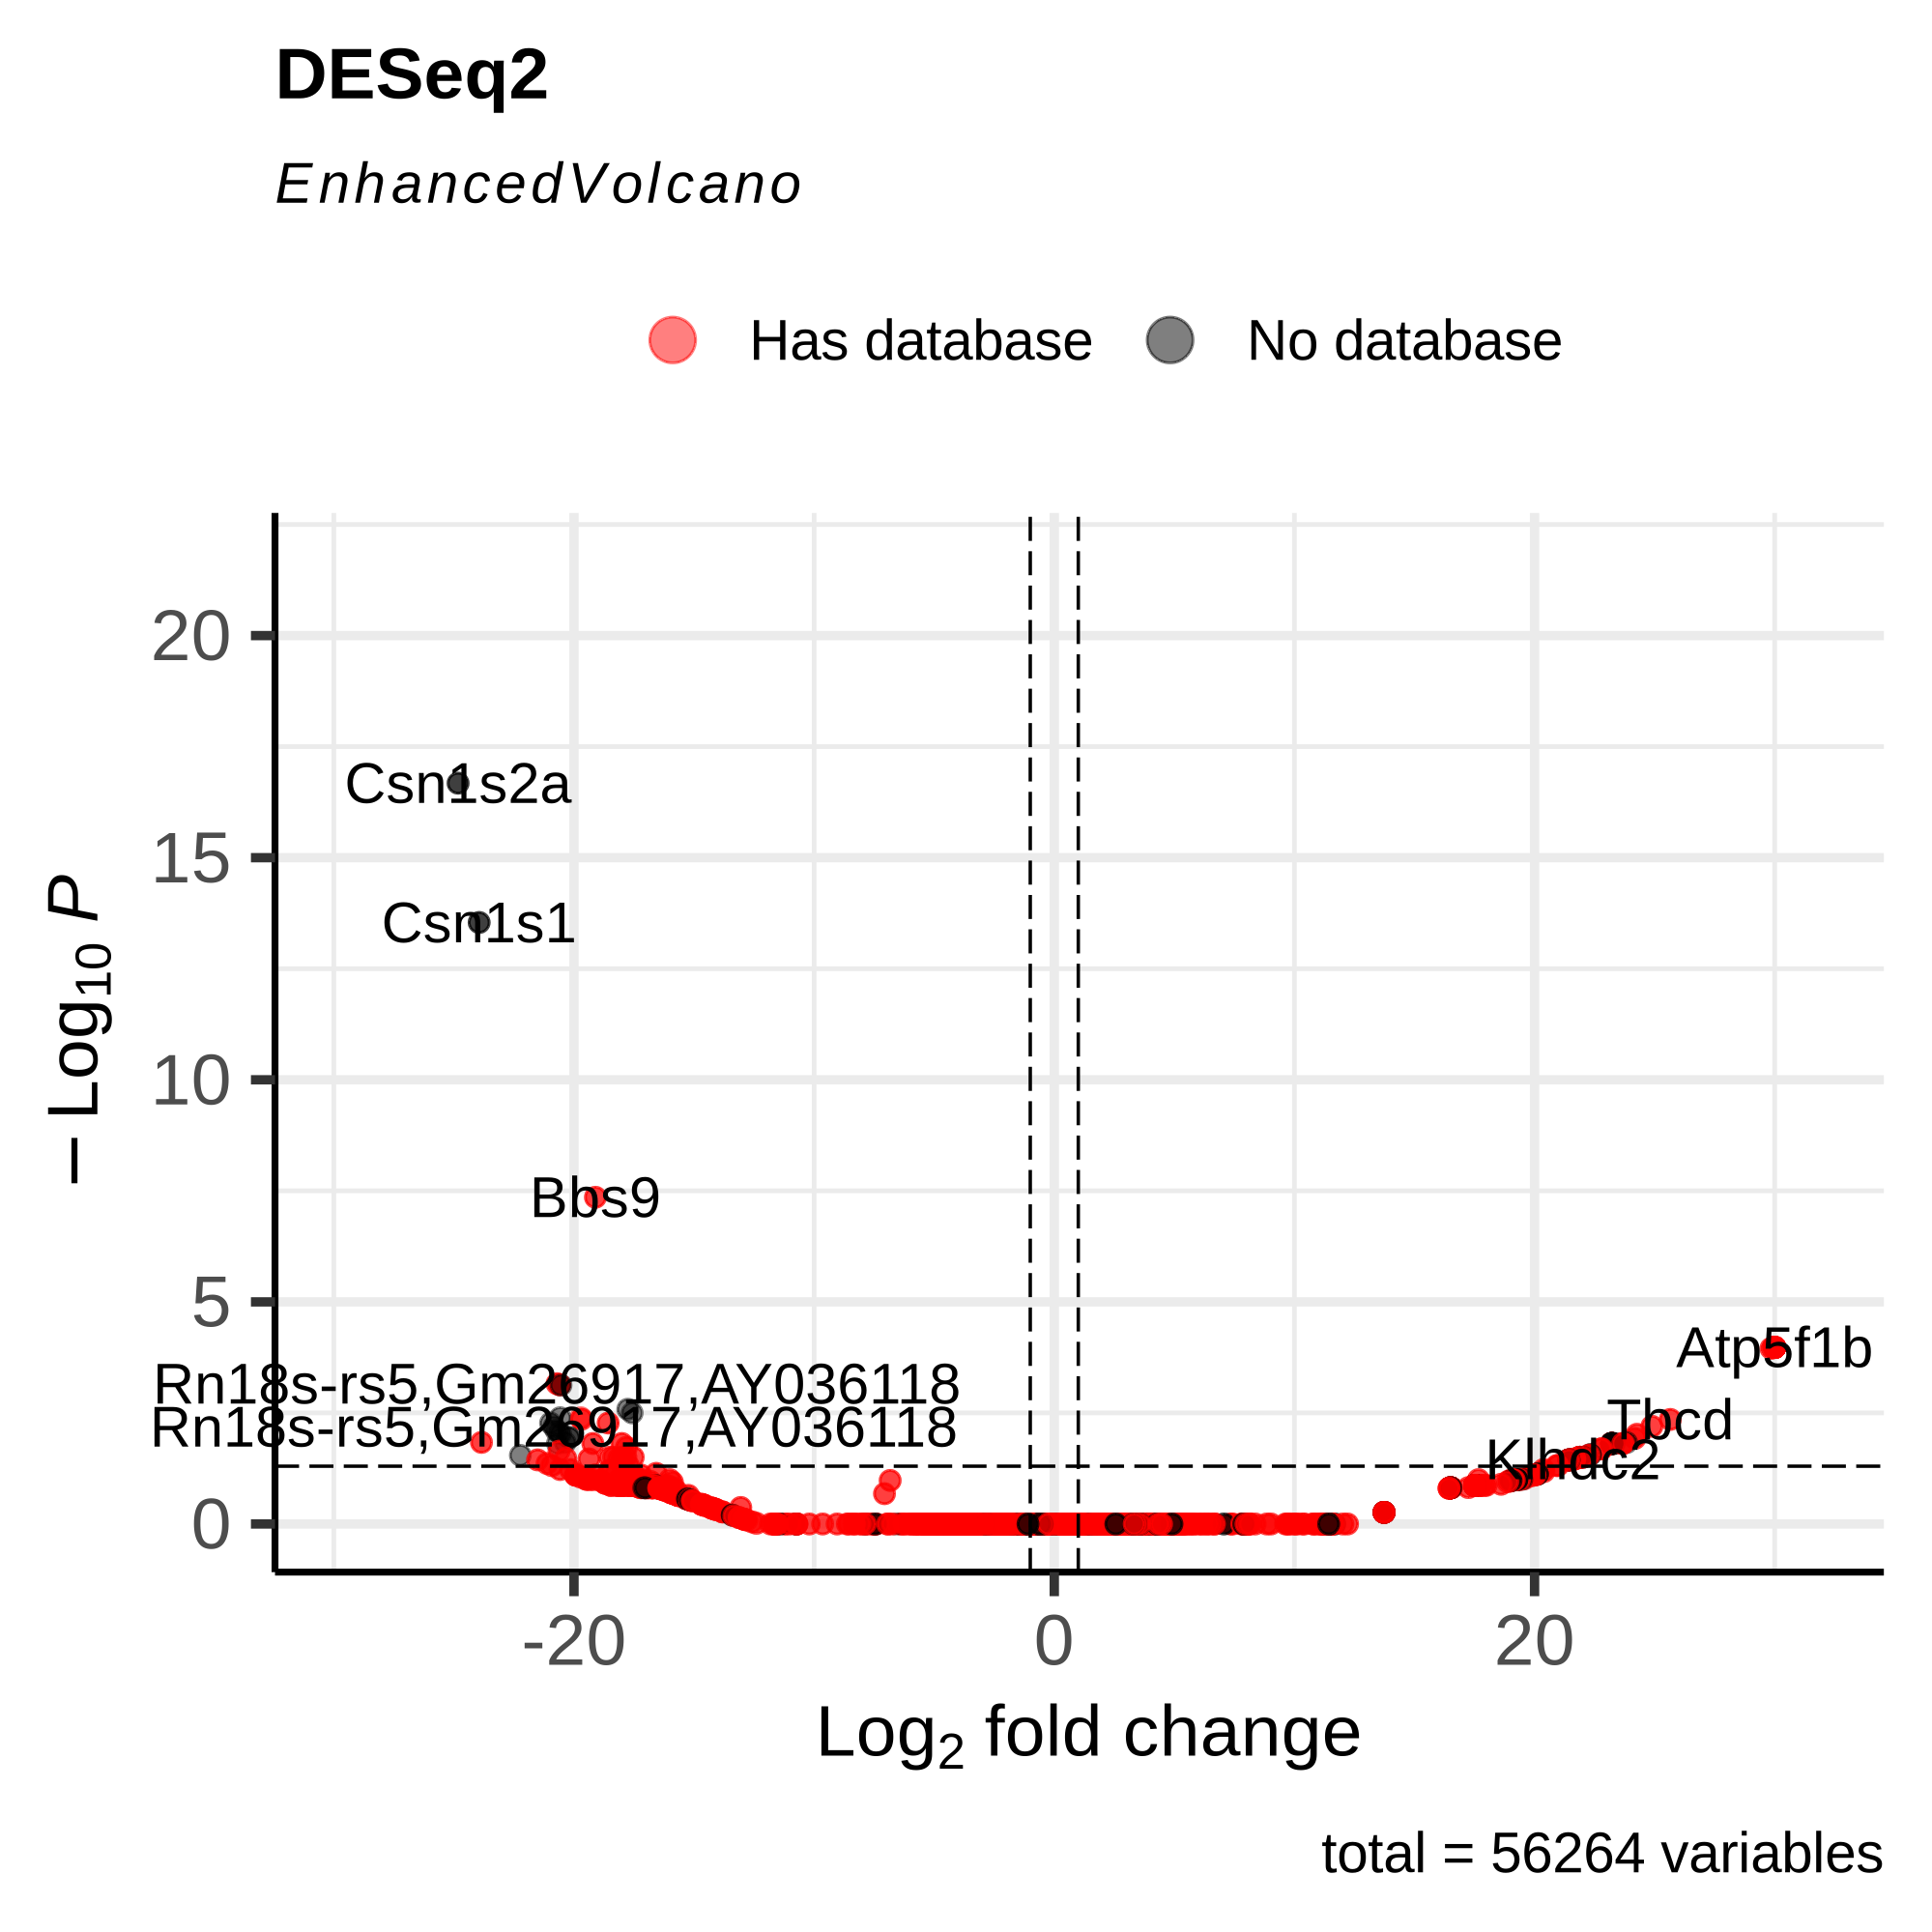
\includegraphics[width=\linewidth]{chapters/4_results_and_discussion/figures/dea/deseq2/letrozole/volcano.png}
                 \caption{Volcano plot illustrating the differential expression
                     results obtained using DESeq2.
                     The same setup as in \cref{fig:tamoxifen_volcano_deseq2} was used.
                 }
                 \label{fig:letrozole_volcano_deseq2}
             \end{subfigure}
        \begin{subfigure}{0.5\textwidth}
            \centering

            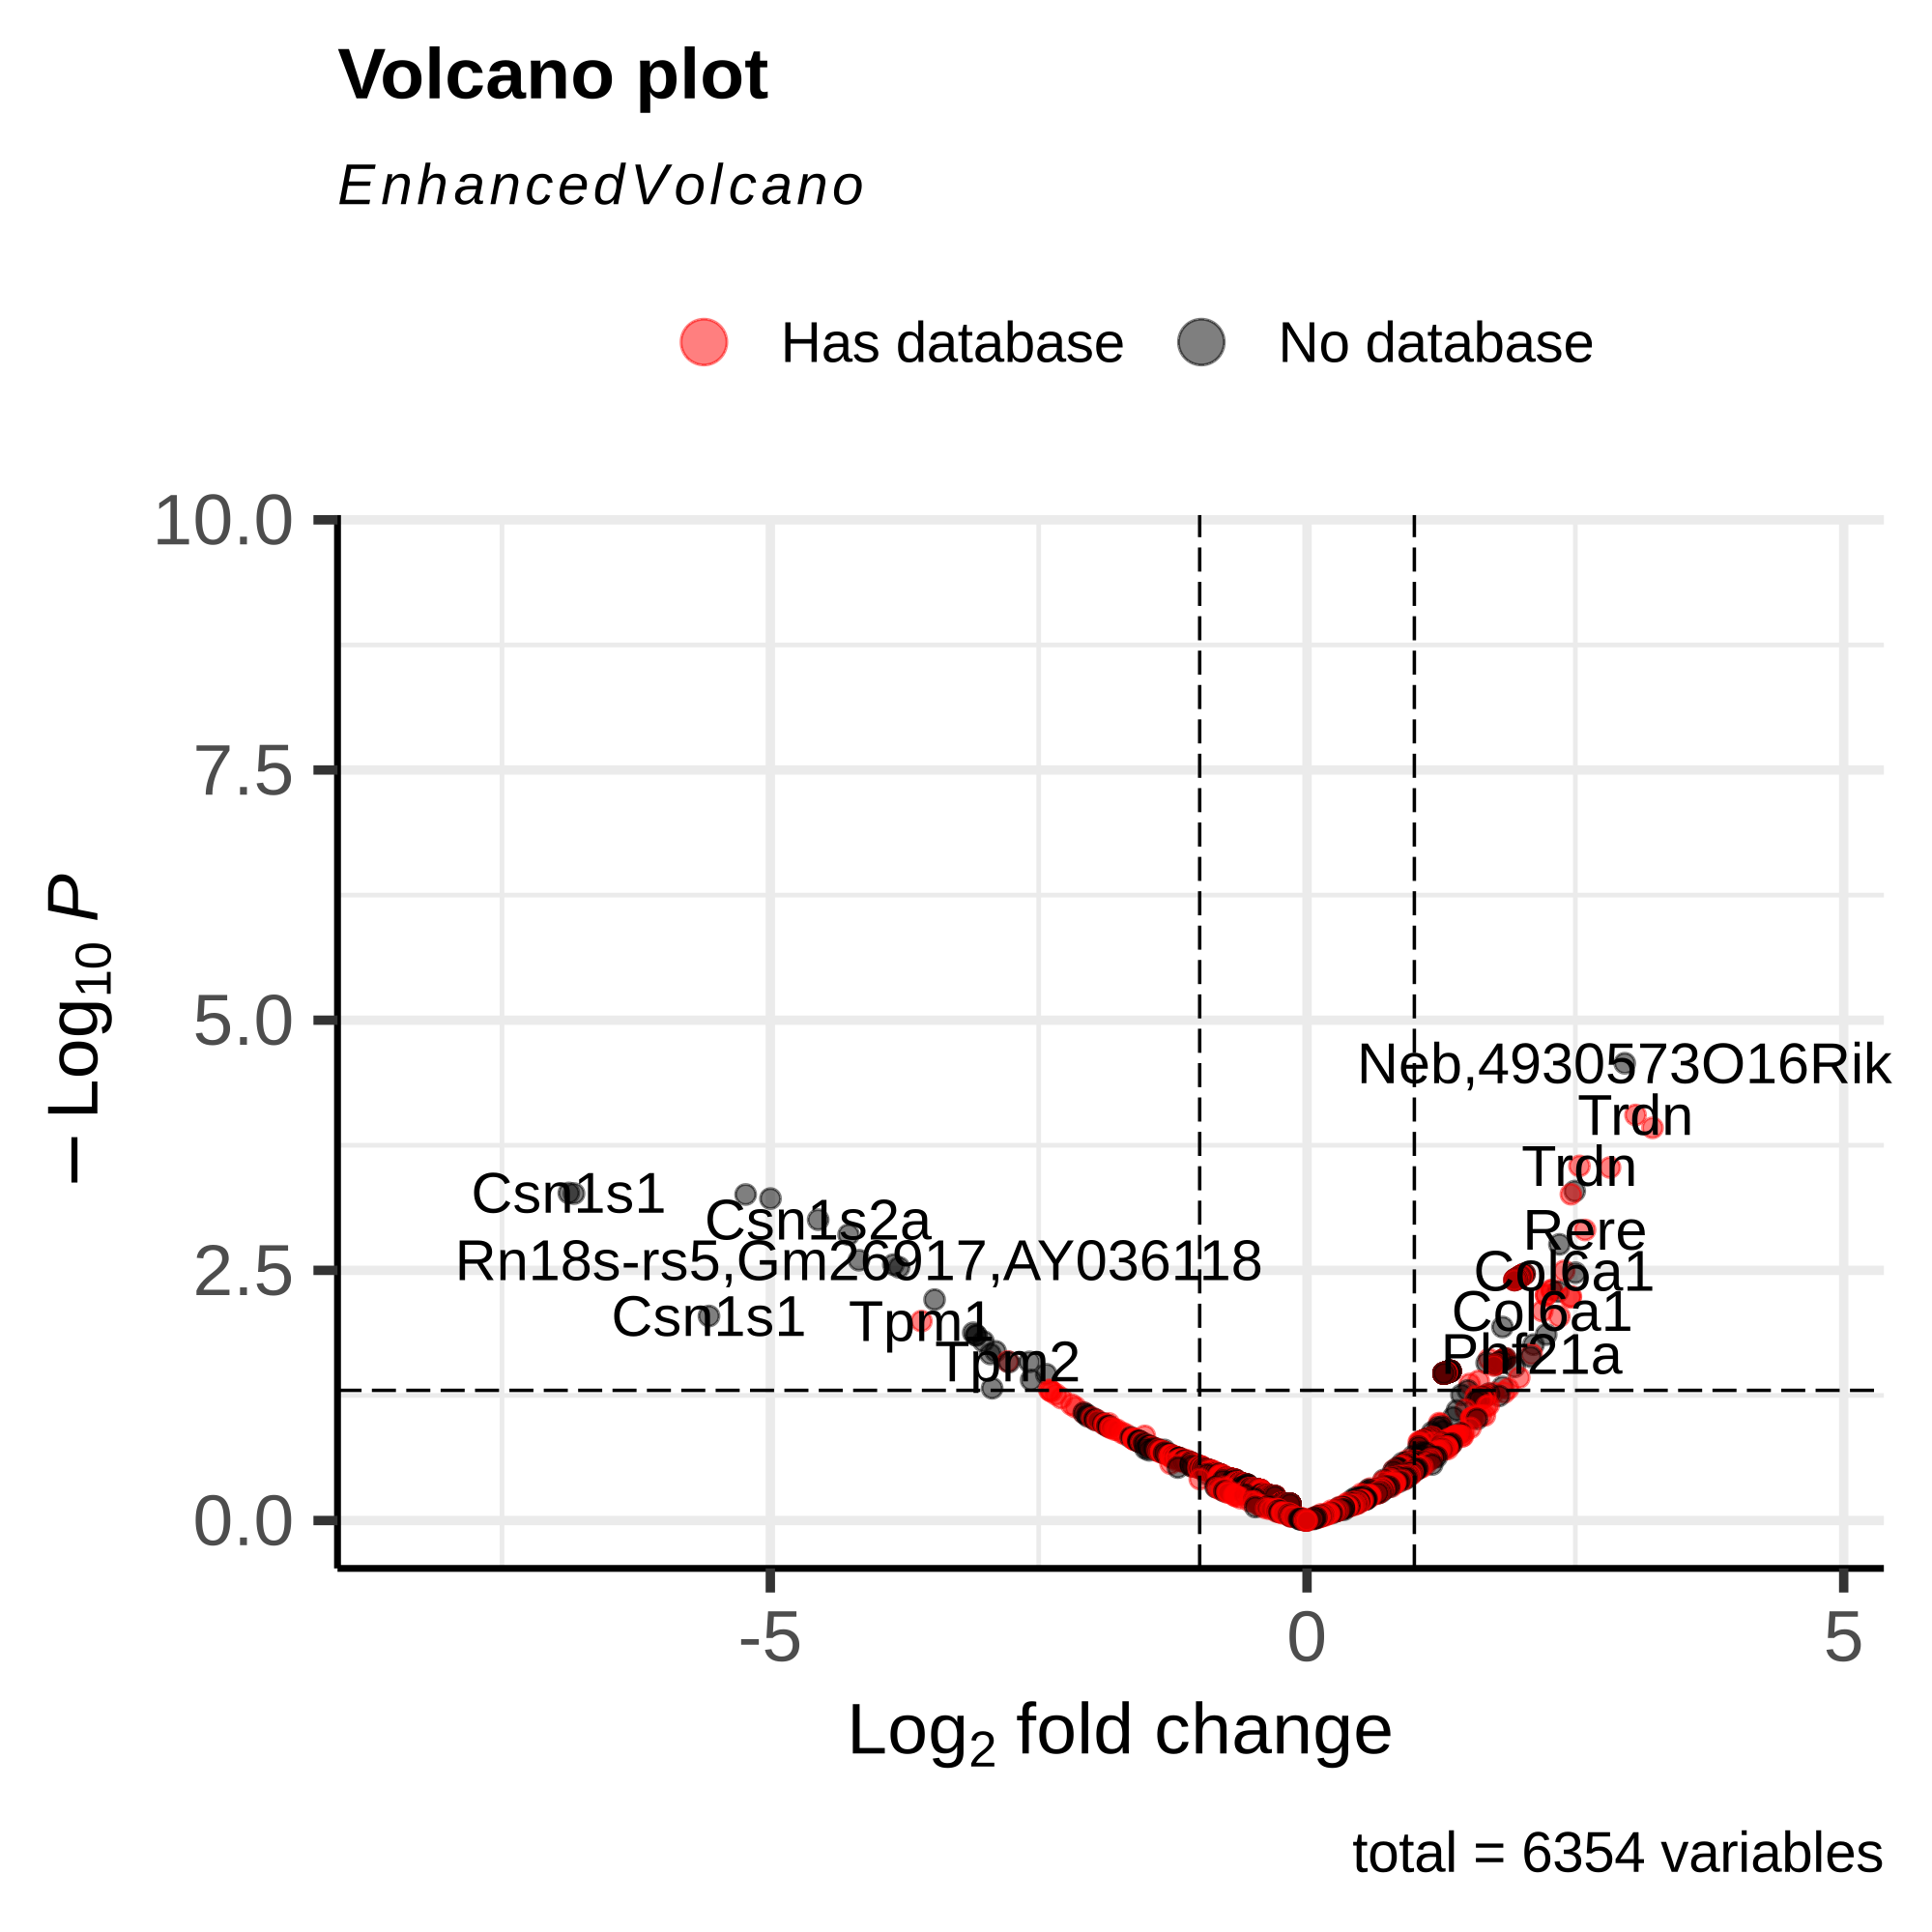
\includegraphics[width=\linewidth]{chapters/4_results_and_discussion/figures/dea/ciriquant/letrozole/volcano.png}
            \caption{Volcano plot illustrating the differential expression
                results obtained using \gls{ciriquant}.
                Samples without treatment were used as the control group, and samples treated
                with \gls{let} were used as the treatment group.
            }
            \label{fig:letrozole_volcano_ciriquant}
        \end{subfigure} &

    \end{tabular}
    \caption{Results of differential expression analysis using the same
        approach as in
        \cref{fig:tamoxifen_volcano}, but comparing samples treated with
        \gls{let}
        to untreated samples.
    }
    \label{fig:letrozole_volcano}
\end{figure}

\subsubsection{Potential target genes}
